% vim: sw=4 ts=4 et
\documentclass[a4paper,12pt]{book}
\usepackage[utf8]{inputenc}
\usepackage{graphicx}
\usepackage{tikz}
\usetikzlibrary{arrows,shapes.geometric,shapes.gates.logic.US,automata,calc,positioning}
\usepackage[style=verbose-ibid,backend=biber]{biblatex}
\usepackage{hyperref}
\usepackage{capt-of}
\usepackage{afterpage}
\usepackage{array}
\usepackage{intcalc}
\usepackage{ifthen}

\sloppy
% From the RISC-V manual
% Commands for register format figures.

% New column types to use in tabular environment for instruction formats.
% Allocate 0.18in per bit.
\newcolumntype{I}{>{\centering\arraybackslash}p{0.18in}}
% Two-bit centered column.
\newcolumntype{W}{>{\centering\arraybackslash}p{0.36in}}
% Three-bit centered column.
\newcolumntype{F}{>{\centering\arraybackslash}p{0.54in}}
% Four-bit centered column.
\newcolumntype{Y}{>{\centering\arraybackslash}p{0.72in}}
% Five-bit centered column.
\newcolumntype{R}{>{\centering\arraybackslash}p{0.9in}}
% Six-bit centered column.
\newcolumntype{S}{>{\centering\arraybackslash}p{1.08in}}
% Seven-bit centered column.
\newcolumntype{O}{>{\centering\arraybackslash}p{1.26in}}
% Eight-bit centered column.
\newcolumntype{E}{>{\centering\arraybackslash}p{1.44in}}
% Ten-bit centered column.
\newcolumntype{T}{>{\centering\arraybackslash}p{1.8in}}
% Twelve-bit centered column.
\newcolumntype{M}{>{\centering\arraybackslash}p{2.2in}}
% Sixteen-bit centered column.
\newcolumntype{K}{>{\centering\arraybackslash}p{2.88in}}
% Twenty-bit centered column.
\newcolumntype{U}{>{\centering\arraybackslash}p{3.6in}}
% Twenty-bit centered column.
\newcolumntype{L}{>{\centering\arraybackslash}p{3.6in}}
% Twenty-five-bit centered column.
\newcolumntype{J}{>{\centering\arraybackslash}p{4.5in}}

\newcommand{\instbit}[1]{\mbox{\scriptsize #1}}
\newcommand{\instbitrange}[2]{~\instbit{#1} \hfill \instbit{#2}~}
\newcommand{\reglabel}[1]{\hfill {\tt #1}\hfill\ }

\newcommand{\wiri}{\textbf{WIRI}}
\newcommand{\wpri}{\textbf{WPRI}}
\newcommand{\wlrl}{\textbf{WLRL}}
\newcommand{\warl}{\textbf{WARL}}

% Code style
\usepackage{listings}
\usepackage{color}
\definecolor{lightgray}{gray}{0.9}

\lstset{
    showstringspaces=false,
    basicstyle=\ttfamily,
    keywordstyle=\color{blue},
    commentstyle=\color[grey]{0.6},
    stringstyle=\color[RGB]{255,150,75}
}

%Local styles
\newcommand{\inlinecode}[2][Verilog]{\lstinline[language=#1]{#2}}

% Flow chart, thanks to Overleaf
% https://www.overleaf.com/learn/latex/LaTeX_Graphics_using_TikZ:_A_Tutorial_for_Beginners_(Part_3)%E2%80%94Creating_Flowcharts
\tikzstyle{startstop} = [rectangle, rounded corners, minimum width=3cm, minimum height=1cm,text centered, draw=black, fill=red!30]
\tikzstyle{io} = [trapezium, trapezium left angle=70, trapezium right angle=110, minimum width=3cm, minimum height=1cm, text centered, draw=black, fill=blue!30]
\tikzstyle{process} = [rectangle, minimum width=3cm, minimum height=1cm, text centered, draw=black, fill=orange!30]
\tikzstyle{decision} = [diamond, minimum width=3cm, minimum height=1cm, text centered, draw=black, fill=green!30]


%\setcounter{secnumdepth}{3}
%\setcounter{tocdepth}{3}
\usepackage{prettyref}
\usepackage{units}
\usepackage{amsmath}

\addbibresource{./references.bib}
\begin{document}

\author{John R. Moser}
\title{The Kerberos RISC-V Core}
\date{May 2020}

\frontmatter
\maketitle
\chapter*{Preface}
This book documents the design of the Taiga and Kerberos RISC-V cores.  Kerberos implements RV32I and RV64I, plus the multiply and divide extension, atomics, single- and double-precision floating point operations, 16-bit compressed instructions, Zicsr, and Zifenci.  Together, this is called RV64IMAFDCZicsr\_Zifencei, or RV32-, etc..  Kerberos also implements SMT, runahead, and out-of-order execution, along with the Supervisor and User modes.

I created Kerberos largely to understand CPU design.  This lead to reading many research papers, learning VHDL and SystemVerilog, and taking lessons from projects such as ZipCPU and the Taiga RISC-V core.  The blog for ZipCPU provided lots of information, but the developers of the Taiga CPU only provided a research paper with not much in-depth detail, along with some follow-up writings.  Because Taiga is so interesting, I decided to look more deeply into it in particular and document lessons learned from its implementation.

Chapters in this book may be short, rather than combined simply for length.  What is topical is topical, and there's no sense in mashing a bunch of different topics together to make a chapter twelve pages long.

I divided this book into three sections:  one reviewing prior work; a sizable section documenting Taiga RISC-V by Matthews and Shannon; and a section documenting the design of Kerberos.
\cleardoublepage
\tableofcontents

\mainmatter
\part{Prior Work}
\chapter{Prior Soft Processors}

Soft processors are common today, provided as synthesizable hardware definition
language (HDL) code and typically deployed to field programmable gate arrays
(FPGA)—although the term "FPGA" is a misnomer, as the device is a fabric of
complex logic elements and not simple gates.  Modern FPGAs provide hard blocks,
including arithmetic logic units (ALU), memory and peripheral bus controllers,
and even entire hard processor systems (HPS) providing a complete
system-on-chip (SOC).

Soft processors implement custom and specialized low-area designs, historic
video game systems, and even large and complex RISC-V processors.  An
engineering firm can convert a soft processor's HDL design into a hard
processor, achieving higher clock rates and lower power usage; while an FPGA
allows rapid testing of different designs to reduce relative delay and power
usage, either for deployment to FPGA or for eventual translation to ASIC.

Kerberos was inspired by and builds on lessons from three soft processors in
particular:  ZipCPU, iDEA, and Taiga.

\section{ZipCPU}

Gisselquist Technology, LLC maintains a blog\footcite{ZipCPU.Blog} discussing
CPU design and their own ZipCPU.  ZipCPU uses its own instruction set
architecture (ISA), aiming for small size, low power, and fast execution.
Gisselquist licenses ZipCPU under GPLv3, with commercial licensing options.

\section{iDEA}

As is typical of anyone who dedicates time, energy, and passion to a subject,
HuiYan Cheah has produced an enormous amount of research and practical work in
the field of digital design.  Cheah's Ph.D thesis, "The iDEA
Architecture-Focused FPGA Soft Processor," thoroughly documents a soft
processor designed to obtain maximum performance from Xilinx FPGAs.  Like
ZipCPU, iDEA implements a custom ISA, in this case heavily leveraging the
DSP48E1 ALU block provided in Xilinx FPGAs.

Cheah achieved a 453MHz clock rate on both a Xilinx Virtex-6 XC6VLX240T-2 and
an Artix-7.

\section{Taiga}

Matthews and Shannon released Taiga, a RISC-V implementation, under the Apache
License 2.0.  They present a high-level overview of Taiga in two
papers\footcite{Matthews2017}\footcite{Matthews2017b}; little deeper detail is
given about Taiga outside the actual published HDL.

\chapter{Adders}

Kerberos provides several adder implementations, including a basic inferred
adder.

\section{Speculative Adders}

Kerberes provides a speculative Han-Carlson adder, a parallel prefix adder with
an enhancement described by Katyayani and many others.  Speculative parallel
prefix adders typically skip the last Kogge-Stone row of a hybrid adder.  This
row propagates a carry half the entire bit width of the adder, not only adding
an extra layer but creating demanding routing.

Parallel prefix adders forward carry bits by stages, with the current
propagated and generated bits forwarding to the next stage.  For example, a
16-bit Han-Carlson passes its bit zero carry directly to bits 1, 3, 7, 15, and
2 in successive stages, in that order.  This propagation functions by specific
rules:

\begin{itemize}
    \item The stage produces a generated carry from the current bit if the
    previous stage produced a generated carry {\em or} if both the previous
    stage produced a propagated carry and the bit propagating its carry to the
    current bit in this stage produced a generated carry in the previous stage.

    \item The stage produces a propagated carry from the current bit if the
    previous stage produced a propagated carry {\em and} the bit propagating
    its carry to the current bit in this stage produced a propagated carry
    in the previous stage.
\end{itemize}

Together, this means a bit permanently generates a carry in all stages after it
generates its first {\em and} a bit permanently propagates no carry in any
stage after it propagates no carry.  No matter how little information you have,
the state of generating and not propagating a carry is permanent.  Notably, any
bit which is 1 in both addends generates a carry and propagates no carry
immediately and is unaffected by all carry propagation.

The penultimate row—the last Kogge-Stone stage—directly propagates any
generated or propagated carry from bit 1 to bit 9, from bit 3 to bit 11, from
bit 5 to bit 13, and from bit 7 to bit 15.  By this time, ever other
propagation has occurred, creating an enormous likelihood of no state change in
this stage.  A high-speed detection circuit operates in parallel with the final
row, the final sum computation, and the parallel computation of the sum {\em
with} the omitted stage.  This introduces a small amount of delay, and in total
the adder can finish in $\frac{4}{5}$ the time, allowing a faster CPU clock
speed if it happens to be the slowest thing in the CPU.  If it detects error,
it signals that addition is incomplete, and provides the correct sum in the
next cycle.

It is possible to cut further rows away; the error rate rapidly increases, but
may be worthwhile on RV128I where the adder has 15\% more delay than a 64-bit
adder.  Kumari, Srinivas, and Aravind find a 64-bit non-speculative Han-Carlson
adder slightly-faster than the inferred adder using the '+' operator in Xilinx
XST.

\section{Carry-Select Adders}

Carry-select adders implement two sets of adders, each for smaller operations,
and each assuming a carry or no carry.  A speculative adder is a complex type
of carry-select adder duplicating a small part of the adder.

Carry-select adders avoid long propagation, such as with ripple-carry adders.
Optimally, a carry-select adder starts with a small adder, then adds larger and
larger adders:  the carry bit switches on the carry bit from the next adder and
switches the output, and that cascades and so gives each successive adder
slightly more time to compute its result, thus allows each stage to be slightly
larger and compute more bits.

\chapter{Dividers}
Dividers use arithmetic facilities to perform integer division.  Dividers are
complex and use algorithms based on repeat subtraction or multiplication.

\section{Quick-Div}
Matthews, Lu, Fang, and Shannon describe Quick-Div in "Rethinking Integer
Divider Design for FPGA-Based Soft-Processors."  This divider can operate at
426MHz on a Xilinx XCVU9P, keeping up with the Taiga RISC-V soft CPU at 373MHz.
The divider is variable-latency and can complete early, freeing up the resource
for further operations.

Quick-Div uses a Count Leading Zero (CLZ) circuit to shift the divisor before
entering the division cycle.  The naive implementation has too much delay, and
so they developed an optimized version.  From there, Quick-Div essentially
implements partial subtraction.  Besides operating at a relatively high clock
rate, it tends to produce more instructions per clock (IPC) than typical
low-radix implementations, and use much less area than high-radix
implementations.

\section{Paravartya}

Jain, Pancholi, Garg, and Saini describe two binary dividers in "Binary
Division Algorithm and High Speed Deconvolution Algorithm." The actual division
computation requires one round per dividend bit minus the number of divisor
bits, and then again minus one.

A Paravartya implementation can use Quick-Div's CLZ to left-align the divisor
and dividend.  Its worst case is division by three:  division by one ultimately
comes down to no operation and a quotient with as many digits as the dividend,
while division by any figure containing a single 1 bit—a power of two—produces
a zero operand of some length, but ultimately of no effect, with the quotient
separated from the remainder by a shift with overflow.

The largest complication with Paravartya is the final barrel shift:  the
dividend begins right-aligned, and the quotient and remainder come out as a
single chunk.  A shift right by the number of digits in the divisor produces
the quotient; an AND produces the remainder.  The quotient is easy enough; the
remainder requires barrel-shifting -1 right to mask the result.

\chapter{Cache Mechanisms}

Caching faces complex concerns:  delay, synonym detection, the precise manner
of tagging, security issues such as seen in recent speculative execution
vulnerabilities, and more.

\section{NCOR}

In 2012, Aasaraai and Moshovos published "NCOR:  An FPGA-Friendly Nonblocking
Data Cache for Soft Processors with Runahead Execution."  Nonblocking cache
allows instruction-level parallelism and specifically allows runahead
execution, wherein a CPU waiting for a cache miss—possibly long enough to
execute several tens or hundreds of instructions—can run instructions with
incorrect data and discard the results just to figure out what data will be
fetched.  A load-store architecture like RISC-V accesses memory infrequently
while executing, so long as the instruction cache can provide the next several
instructions.  Runahead discards the results of instructions, but queues data
cache loads as best it can predict so they occur while the CPU executes
preceding instructions.  Runahead can often generate confirmed correct
computations, notably for branches, providing a high-accuracy branch predictor.

Runahead does particularly interesting things when encountering loops:  if it
can properly predict valid load addresses within the loop—such as by tracking
an increment—it can rapidly identify further data with high accuracy.  If
runahead produces erroneous results, a cache miss will occur when entering the
loop; once inside the loop, this information is definitely correct, and
runahead generally predicts the correct results.

NCOR provides a non-blocking cache which avoids content-addressable memory and
leverages FPGA resources such as BRAM.  It reaches fMax of over 325MHz on a
Spartan III with a 4KiB cache, versus 200MHz for a stripped-down MSHR-based
cache.  Both architectures spend more time slogging through larger caches, with
NCOR running at 300MHz on both 8KiB and 16KiB cache sizes, and near 275MHz on
32KiB.  Separate instruction and data caches with slower (multi-cycle, low
delay but longer latency) L2 cache allow higher fMax when the cache
infrastructure is in the critical path, which means more runahead distance and
fewer cache misses.

\section{VC-DSR}

Most L1 caches are virtually-indexed, physically-tagged (VIPT).  This requires
a TLB lookup on each cache access, possible page table walking, and other slow
behavior.  The TLB lookup itself induces longer delays.  Virtually-indexed,
virtually-tagged (VIVT) caches can encounter multiple virtual addresses (VAs)
with the same physical address, called synonyms.

Yoon and Sohi proposed\footcite{Yoon2016} a Virtual Cache with Dynamic Synonym
Remapping (VC-DSR), as shown in \prettyref{fig:VC-DSR}.  This solves the
synonym probleh in VIVT by looking up synonyms in an Active Synonym Table (AST)
if a virtual address matches a Synonym Signature (SS), implemented as a bloom
filter.  If no SS or AST hit, it checks the VC as normal.  When multiple cached
virtual pages map to the same physical page, the AST provides the Leading
Virtual Page (LVP) used to look up the address in the VC, as well as the
permissions and other metadata for that particular virtual page.  The cache
then looks up the tag for the leading virtual page—logically, it replaces the
bits in the virtual address with the bits of the leading virtual page,
producing the Leading Virtual Address (LVA), and uses that to find the cache
line; the L1 arbiter ignores the metadata in this cache entry, using the data
from the AST instead.

\begin{figure}[hbpt]
    \centering
    \includegraphics[width=\textwidth]{images/VC-DSR_Cache}
    \caption{\label{fig:VC-DSR}VC-DSR as diagramed by Yoon and Sohi, with LLVP added.}
\end{figure}

On VC miss, the TLB checks the Active Synonym Detection Table (ASDT) to
determine if the virtual page is known to correspond to a physical page in
cache.  If not, the caching system makes further requests to L2 cache or
performs a page table walk.  If the virtual page ultimately does reference a
physical page already in cache, the cache arbiter hashes the page, sets the
corresponding bit in SS, increments a counter for this bit, and inserts the
virtual page into the AST as a synonym to the LVP.

The Last LVP (LLVP) optimization, shown in \prettyref{fig:VC-DSR}, stores the
last leading virtual page and requested page in a register, along with
metadata.  If the requested address matches the last requested address, the
cache arbiter can immediately check metadata (read or write permission) and mux
the LVP from this register.  Consecutive memory accesses to the same synonym
page skip the AST check; the SS check occurs in parallel, but adds no delay and
has no effect.

RISC-V provides a Global bit in the PTE.  The cache arbiter ignores the ASID
for Global pages, placing no entry in the SS or AST for the same virtual page
in different ASIDs.  Synonyms mapped at alternate virtual addresses are treated
as normal.  On IA-32 and AMD64, Yoon and Sohi assume the top half of virtual
address space is global.

%\part{The Taiga RISC-V Soft Processor}
\chapter{Taiga}

Eric Matthews and Lesley Shannon created Taiga "to facilitate research into heterogeneous processor systems and high performance architectural features for soft processors."  Their goals included high instruction-level paralelization (ILP) at competitive operating frequencies (fMax) and area usage.

In 2017, Taiga ran on a Xilinx Zynq X7CZ020 FPGA at 111MHz in its minimal without multiply, divide, TLB, MMU, cache, or atomic operations, and 103MHz at full configuration.  This version also achieved 254MHz on a Xilinx Virtex UltraScale+ XCVU9P.  The critical path was the write-back data path in all except the full configuration, which was limited by access to data TLB tags.

In 2019, they tested Quick-Div on a Xilinx Virtex UltraScale+ VCU118 FPGA board using an XCVU9P-L2FLGA2014E.  They needed Quick-Div to run at 373MHz to stay out of the critical path—just shy of 50\% higher fMax than they achieved on the XCVU9P in 2017.  Clearly, they have improved the processor over time.

Nearly 400MHz performance, even on a modern FPGA, is impressive.  Taiga achieves clock rates comparable to iDEA, yet implements a full RV32 RISC-V processor capable of running Linux.

%I aim to document Taiga here so as to facilitate independent learning.  Digital design is highly-accessible with free tools and low-cost development boards for high-performance FPGAs and FPGA-SoCs; and more importantly, while nobody is going to engineer a modern high-end processor from what they read on Wikipedia, it's ridiculously easy for the average person with no background in digital design to learn an HDL and design a CPU.  Skills from programming translate well, so long as you can get your head around combinational logic—that is, a logic block where everything happens continuously—and latched signals.  Whereas programs execute sequentially, combinational logic executes continuously, such that changes propagate at the speed of electrical signals to change the outcome.  A firm understanding of this concept allows competent exploration of digital design.
\part{Kerberos}
\chapter{Overview}

\prettyref{fig:Kerberose-block-diagram-overview} shows a high-level overview of
the Kerberos processor.


\begin{figure}
% Kerberos overview, similar to Taiga diagram
    \begin{center}
        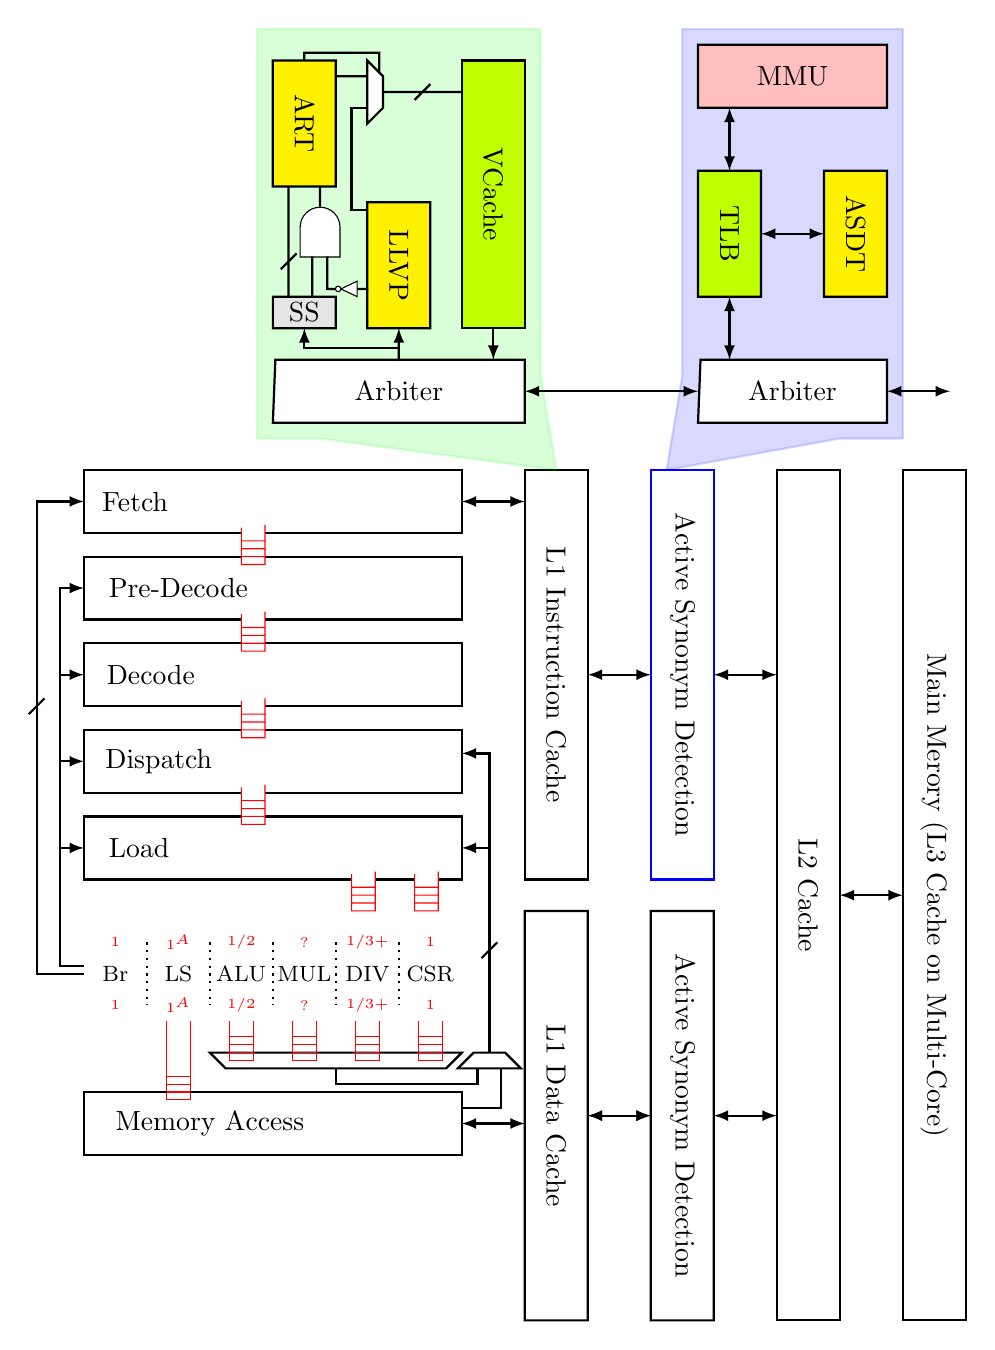
\begin{tikzpicture}[scale=0.2]
            \tikzstyle{every node}+=[inner sep=0pt]

            % Fetch
            \path
                 % Outer rectangle
                 [black,draw,thick]
                 % Origin
                 (0,0) node [black] (Fetch) {}
                 % Label
                 (Fetch) ++(3.25,-2) node [black] {Fetch}
                 % Box
                 (Fetch)
               ++(10,-4) -- ++(-10,0) -- ++(0,4) -- ++(24,0) -- ++(0,-4) -- ++(-12.5,0)
                 % Pipeline position
                 (Fetch) ++(10,-3.5) node (FetchPL1) {};

            % Pre-Decoder
            \path
                [black, draw, thick]
                % Origin, relative to Fetch
                (Fetch) ++(0,-5.5) node (PreDecode) {}
                (PreDecode) ++(6,-2) node {Pre-Decode}
                % Box
                (PreDecode)
                (FetchPL1) ++(0,-2)
                -- ++(-10,0) -- ++(0,-4) -- ++(10,0)
              ++(1.5,0) -- ++(12.5,0) -- ++(0,4) -- ++(-12.5,0)
                (PreDecode) ++(10,-3.5) node (PreDecodePL1) {};

            % Decoder
            \path
                [black, draw, thick]
                % Origin, relative to Fetch
                (PreDecode) ++(0,-5.5) node (Decode) {}
                (Decode) ++(4.25,-2) node {Decode}
                % Box
                (Decode)
                (PreDecodePL1) ++(0,-2)
                -- ++(-10,0) -- ++(0,-4) -- ++(10,0)
              ++(1.5,0) -- ++(12.5,0) -- ++(0,4) -- ++(-12.5,0)
                (Decode) ++(10,-3.5) node (DecodePL1) {};

            % Ordering
            \path
                [black, draw, thick]
                % Origin, relative to Fetch
                (Decode) ++(0,-5.5) node (Order) {}
                (Order) ++(4.75,-2) node {Dispatch}
                % Box
                (Order)
                (DecodePL1) ++(0,-2)
                -- ++(-10,0) -- ++(0,-4) -- ++(10,0)
              ++(1.5,0) -- ++(12.5,0) -- ++(0,4) -- ++(-12.5,0)
                (Order) ++(10,-3.5) node (OrderPL1) {};

            % Load
            \path
                [black, draw, thick]
                (Order) ++(0,-5.5) node (Load) {}
                (Load) ++(3.5,-2) node {Load}
                (OrderPL1) ++(0,-2)
              -- ++(-10,0) -- ++(0,-4) -- ++(17,0)
              ++(0,0.5) node (LoadPL1) {}
              ++(1.5,-0.5) -- ++(2.5,0) ++(0,0.5) node (LoadPL2) {}
              ++(1.5,-0.5) -- ++(1.5,0) -- ++(0,4) -- ++(-12.5,0);

            %%%%%%%%%%%%%%%%%
            % Execute phase %
            %%%%%%%%%%%%%%%%%

            \path (Load) ++(0,-8) node (ExecutePhase) {};

            \path
                [black, draw, thick, text centered]
                (ExecutePhase) node (ExBranch) {}
              ++(2,-2) node {\footnotesize{Br}}
                (ExBranch) ++(2,0) node [red] {\tiny{1}}
              ++(0,-4) node [red] {\tiny{1}};
            \path
                [black, draw, thick, text centered]
                (ExBranch) ++(4,0) node (ExLS) {}
              ++(2,-2) node {\footnotesize{LS}}
                (ExLS) ++(2,0) node [red] {\tiny{$1^A$}}
              ++(0,-4) node [red] {\tiny{$1^A$}};
            \path
                [black, draw, thick, text centered]
                (ExLS) ++(4,0) node (ExALU) {}
              ++(2,-2) node {\footnotesize{ALU}}
                (ExALU) ++(2,0) node [red] {\tiny{1/2}}
              ++(0,-4) node [red] {\tiny{1/2}};
            \path
                [black, draw, thick, text centered]
                (ExALU) ++(4,0) node (ExMUL) {}
              ++(2,-2) node {\footnotesize{MUL}}
                (ExMUL) ++(2,0) node [red] {\tiny{?}}
              ++(0,-4) node [red] {\tiny{?}};
            \path
                [black, draw, thick, text centered]
                (ExMUL) ++(4,0) node (ExDIV) {}
              ++(2,-2) node {\footnotesize{DIV}}
                (ExDIV) ++(2,0) node [red] {\tiny{1/3+}}
              ++(0,-4) node [red] {\tiny{1/3+}};
            \path
                [black, draw, thick, text centered]
                (ExDIV) ++(4,0) node (ExCSR) {}
              ++(2,-2) node {\footnotesize{CSR}}
                (ExCSR) ++(2,0) node [red] {\tiny{1}}
              ++(0,-4) node [red] {\tiny{1}};
            \path
                [black, draw, thick, dotted]
                (ExBranch)
              ++(4,0) -- ++(0,-4)
                (ExLS)
              ++(4,0) -- ++(0,-4)
                (ExALU)
              ++(4,0) -- ++(0,-4)
                (ExMUL)
              ++(4,0) -- ++(0,-4)
                (ExDIV)
              ++(4,0) -- ++(0,-4);
            % Mux
            \path
                [black, draw, thick]
                (ExALU) ++(1.25,-7)
                node (ExMux) {}
              ++(1.5,0) -- ++(2.5,0)
              ++(1.5,0) -- ++(2.5,0)
              ++(1.5,0) -- ++(2.5,0)
              ++(1.5,0) -- ++(1.25,0)
                -- ++(-1,-1) -- ++(-14,0) -- ++(-1,1) -- ++(1.25,0) -- cycle;
            \path
                [black, draw, thick]
                (ExMux) ++(14.5,-1)
                node (ExMemMux) {}
                ++(1,1) -- ++(2,0) -- ++(1,-1) -- ++(-4,0) -- cycle;
            % Execution unit pipelines
            \foreach \x in {ExALU, ExMUL, ExDIV, ExCSR}
            \path
                [red, draw]
                (\x) ++(1.25,-5) -- ++(0,-2.5) -- ++(1.5,0) -- ++(0,2.5)
                (\x) ++(1.25,-5) -- ++(0,-2) -- ++(1.5,0)
              ++(0,0.5) -- ++(-1.5,0)
              ++(0,0.5) -- ++(1.5,0);

            % LS has a longer reach to the MEM stage
            \path
                [red, draw]
                (ExLS) ++(1.25,-5) -- ++(0,-5) -- ++(1.5,0) -- ++(0,5)
                (ExLS) ++(1.25,-7.5) -- ++(0,-2) -- ++(1.5,0)
              ++(0,0.5) -- ++(-1.5,0)
              ++(0,0.5) -- ++(1.5,0);

            % Mem
            \path
                [black, draw, thick]
                % Origin, relative to Exec
                (ExecutePhase) ++(0,-9.5) node (MemPhase) {}
                (MemPhase) ++(8,-2) node {Memory Access}
                % Box
                (ExLS) ++(1.25,-9.5) -- ++(-5.25,0)
                -- ++(0,-4) -- ++(10,0) -- % No pipeline down, so connect
              ++(1.5,0) -- ++(12.5,0) -- ++(0,4) -- ++(-17.25,0)
                (MemPhase) ++(10,-3.5) node (MemPL1) {};
            % Branch and forward
            \path %Branch
                [->,>=latex,black,draw,thick]
                (ExBranch) ++(0,-2)
                -- ++(-3,0) -- ++(0,30) -- ++(3,0);
            \path %Branch data slash
                [black,draw,thick]
                (ExBranch) ++(-3.5,14.5) -- ++(1,1);
            %%%% Branch Flushes
            \foreach \x in {7.5, 13,18.5,24}
            \path
                [->,>=latex,black,draw,thick]
                (ExBranch) ++(0,-1.5)
                -- ++(-1.5,0) -- ++(0,\x) -- ++(1.5,0);
            %%% End flushes
            \path % Execution MUX to forward MUX
                [black,draw,thick]
                (ExMux) ++(6.75,-1)
                -- ++(0,-1) -- ++(9,0) -- ++(0,1);
            \path
                [black,draw,thick]
                (MemPhase) ++(24,-1)
                -- ++(2.5,0) -- ++(0,2.5);
            \path
                [->,>=latex,black,draw,thick]
                (ExMemMux) ++(2,1)
                -- ++(0,13) -- ++(-1.75,0);
            \path
                [->,>=latex,black,draw,thick]
                (ExMemMux) ++(2,1)
                -- ++(0,19) -- ++(-1.75,0);
            \path % Mux data slash
                [black,draw,thick]
                (ExMemMux) ++(1.5,7) -- ++(1,1);
            % Pipelines
            \foreach \x in {FetchPL1, PreDecodePL1, DecodePL1, OrderPL1, LoadPL1, LoadPL2}
            \path
                [red, draw]
                (\x) -- ++(0,-2.5) -- ++(1.5,0) -- ++(0,2.5)
                (\x) ++(0,-2) -- ++(1.5,0)
                ++(0,0.5) -- ++(-1.5,0)
                ++(0,0.5) -- ++(1.5,0);
            %%%%%%%%%%%%%%%%%%
            % Memory Systems %
            %%%%%%%%%%%%%%%%%%

            % L1 I$
            \path
                [black, draw, thick]
                (Fetch) ++(28,0) node (ICache) {}
              ++(2,-13) node [rotate=-90] {L1 Instruction Cache}
                (ICache)
                -- ++(4,0) -- ++(0,-26) -- ++(-4,0) -- ++(0,26) -- cycle;
            \path
                [<->,>=latex,black,draw,thick]
                (Fetch) ++(24,-2) -- ++(4,0);
            % L1 I$ expansion
            \path
                [fill, draw, thick, green, opacity=0.15]
                (ICache) ++(-16,28) node (ICache Detail) {}
                (ICache Detail) ++(18,-28)
                -- ++(-1,6) -- ++(0,22) -- ++(-18,0) -- ++(0,-26) -- ++(4,0) -- cycle;
            \path
                [black, draw, thick, fill=white]
                (ICache Detail) ++(0,-21) node (ICache Arbiter) {}
              ++(8,-2) node {Arbiter}
                (ICache Arbiter)
                -- ++(16,0) -- ++(0,-4) -- ++(-16,0) -- cycle;
            \path
                [black, draw, thick,fill=lightgray]
                (ICache Arbiter) ++(0,2) node (SS) {}
              ++(2,1) node {SS}
                (SS)
                -- ++(4,0) -- ++(0,2) -- ++(-4,0) -- ++(0,-2) -- cycle;
            \path
                [black, draw, thick, fill=yellow]
                (SS) ++(0,17) node (ART) {}
              ++(2,-4) node [rotate=-90] {ART}
                (ART)
                -- ++(4,0) -- ++(0,-8) -- ++(-4,0) -- ++(0,8) -- ++(4,0) -- cycle;
            \path
                [black, draw, thick, fill=yellow]
                (ICache Arbiter) ++(6,10) node (LLVP) {}
              ++(2,-4) node[rotate=-90] {LLVP}
                (LLVP)
                -- ++(4,0) -- ++(0,-8) -- ++(-4,0) -- ++(0,8) -- cycle;
            \path
                [black, draw, thick, fill=lime]
                (ART) ++(12,0) node (VCache) {}
                ++(2,-8.5) node [rotate=-90] {VCache}
                (VCache)
                -- ++(0,-17) -- ++(4,0) -- ++(0,17) -- ++(-4,0) -- cycle;
            % AND gate
            \node[and gate US, draw,rotate=90, fill=white] at ($(SS) + (3,6)$) (SSAnd) {};
            \node[not gate US, draw, rotate=180, scale=0.5, fill=white] at ($(LLVP) + (-1,-5.5)$) (SSNot) {};
            \path
                [black, draw, thick]
                (SS) ++(2.5,2) |- (SSAnd.input 1)
                (SS) ++(1,2) -- ($(ART) + (1,-8)$)
                (SS) ++(0.5,3.75) -- ++(1,1) % Slash to show multi-data bus
                (LLVP) ++(0,-5.5) |- (SSNot.input) (SSNot.output) -- ++(-0.5,0) |- (SSAnd.input 2)
                (SSAnd.output) -- ($(ART) + (3,-8)$);
            % Mux
            \path
                [black, draw, thick, fill=white]
                (ART) ++(6,0) node (Mux) {}
                -- ++(0,-4) -- ++(1,1) -- ++(0,2) -- cycle;
            \path
                [black, draw, thick]
                (LLVP) ++(0,-0.5) -- ++(-1,0) -- ++(0,6.5) -- ++(1,0);
            \path
                [black, draw, thick]
                (ART) ++(4,-1) -- ++(2,0)
                (ART) ++(2,0) -- ++(0,0.5) -- ($(Mux) + (0.75,0.5)$) -- ++(0,-1.25)
                (Mux) ++(1,-2) -- ($(VCache) + (0,-2)$)
                (Mux) ++(1,-2) ++(2,-0.5) -- ++(1,1); % slashfor wide data
            \path
                [->,>=latex,black,draw,thick]
                (ICache Arbiter) ++(8,0) -- ($(LLVP) + (2,-8)$);
            \path
                [->,>=latex,black,draw,thick]
                (ICache Arbiter) ++(8,0) -- ++(0,0.75) -- ++(-6,0) -- ++(0,1.25);
            \path
                [->,>=latex,black,draw,thick]
                (VCache) ++(2,-17) -- ++(0,-2);


            % Active Synonym Detection layer
            \path
                [blue, draw, thick]
                (ICache) ++(8,0) node (IASD) {}
              ++(2,-13) node [black,rotate=-90] {Active Synonym Detection}
                (IASD)
                -- ++(4,0) -- ++(0,-26) -- ++(-4,0) -- ++(0,26) -- cycle;
            \path
                [<->,>=latex,black,draw,thick]
                (ICache) ++(4,-13) -- ++(4,0);
            % ASD Expansion
            \path
                [fill, draw, thick, blue, opacity=0.15]
                (IASD) ++(2,28) node (IASD Detail) {}
                (IASD Detail) ++(-1,-28)
                -- ++(1,6) -- ++(0,22) -- ++(14,0) -- ++(0,-26) -- ++(-4,0) -- cycle;
            \path
                [black, draw, thick, fill=white]
                (IASD Detail) ++(1,-21) node (IASD Arbiter) {}
              ++(6,-2) node {Arbiter}
                (IASD Arbiter)
                -- ++(12,0) -- ++(0,-4) -- ++(-12,0) -- cycle;
            \path
                [black, draw, thick, fill=lime]
                (IASD Arbiter) ++(0,12) node (TLB) {}
              ++(2,-4) node [rotate=-90] {TLB}
                (TLB)
                -- ++(4,0) -- ++(0,-8) -- ++(-4,0) -- ++(0,8) -- cycle;
            \path
                [black, draw, thick, fill=yellow]
                (TLB) ++(8,0) node (ASDT) {}
              ++(2,-4) node [rotate=-90] {ASDT}
                (ASDT)
                -- ++(4,0) -- ++(0,-8) -- ++(-4,0) -- ++(0,8) -- cycle;
            \path
                [black, draw, thick, fill=pink]
                (TLB) ++(0,8) node (MMU) {}
              ++(6,-2) node {MMU}
                (MMU)
                -- ++(12,0) -- ++(0,-4) -- ++(-12,0) -- ++(0,4) -- cycle;

            \path
                [<->,>=latex,black,draw,thick]
                (ICache Arbiter) ++(16,-2) -- ++(11,0);
            \path
                [<->,>=latex,black,draw,thick]
                (IASD Arbiter) ++(12,-2) -- ++(4,0);
            \path
                [<->,>=latex,black,draw,thick]
                (IASD Arbiter) ++(2,0) -- ++(0,4);
            \path
                [<->,>=latex,black,draw,thick]
                (TLB) ++(4,-4) -- ++(4,0);
            \path
                [<->,>=latex,black,draw,thick]
                (TLB) ++(2,0) -- ++(0,4);

            % L1 D$
            \path
                [black, draw, thick]
                (ICache) ++(0,-28) node (DCache) {}
              ++(2,-13) node [rotate=-90] {L1 Data Cache}
                (DCache)
                -- ++(4,0) -- ++(0,-26) -- ++(-4,0) -- ++(0,26) -- cycle;
                \path
                [<->,>=latex,black,draw,thick]
                (DCache) ++(4,-13) -- ++(4,0);
            \path
                [<->,>=latex,black,draw,thick]
                (MemPhase) ++(24,-2) -- ++(4,0);
            % Active Synonym Detection layer
            \path
                [black, draw, thick]
                (DCache) ++(8,0) node (DASD) {}
              ++(2,-13) node [rotate=-90] {Active Synonym Detection}
                (DASD)
                -- ++(4,0) -- ++(0,-26) -- ++(-4,0) -- ++(0,26) -- cycle;
                \path
                [<->,>=latex,black,draw,thick]
                (DCache) ++(4,-13) -- ++(4,0);

            % L2 Cache
            \path
                [black, draw, thick]
                (IASD) ++(8,0) node (L2 Cache) {}
              ++(2,-27) node [rotate=-90] {L2 Cache}
                (L2 Cache)
                -- ++(4,0) -- ++(0,-54) -- ++(-4,0) -- ++(0,54) -- cycle;
            \path
                [<->,>=latex,black,draw,thick]
                (IASD) ++(4,-13) -- ++(4,0);
            \path
                [<->,>=latex,black,draw,thick]
                (DASD) ++(4,-13) -- ++(4,0);
            % L3 Cache
            \path
                [black, draw, thick]
                (L2 Cache) ++(8,0) node (L3 Cache) {}
                ++(2,-27) node [rotate=-90] {Main Merory (L3 Cache on Multi-Core)}
                (L3 Cache)
                -- ++(4,0) -- ++(0,-54) -- ++(-4,0) -- ++(0,54) -- cycle;
            \path
                [<->,>=latex,black,draw,thick]
                (L2 Cache) ++(4,-27) -- ++(4,0);
        \end{tikzpicture}
    \end{center}
    \label{fig:Kerberose-block-diagram-overview}
\end{figure}

\section{Memory Access and Cache}


\chapter{Pipeline}

\section{Skid Buffer}

I built the Kerberos skid buffer based on excellent explanations at the ZipCPU
blog \footcite{ZipCPU.Pipeline}.  \prettyref{fig:pipeline-skid-buffer-fsm}
shows the state machine for the skid buffer.
\prettyref{tab:skid-buffer-handshake-state} shows information about each state;
as noted on the ZipCPU blog, \inlinecode{$In.Busy = FullBuffer$}.

\afterpage{
\begin{table}[ht]
    \caption{table}{Handshake States} % title of Table
    \centering % used for centering table
    \begin{tabular}{c c c c} % centered columns (4 columns)
        \hline\hline
        State & FullBuffer & Out.Strobe & DataOut \\ [0.5ex] % inserts table

        \hline
        Passthrough & 0 & In.Strobe & Din \\
        Buffer & 1 & In.Strobe & Din \\
        Flush & 0 & 1 & Buffer \\ [1ex]
        \hline
    \end{tabular}
    \label{tab:skid-buffer-handshake-state}
\end{table}

    % Pipeline FSM
\begin{figure}
    \begin{center}
        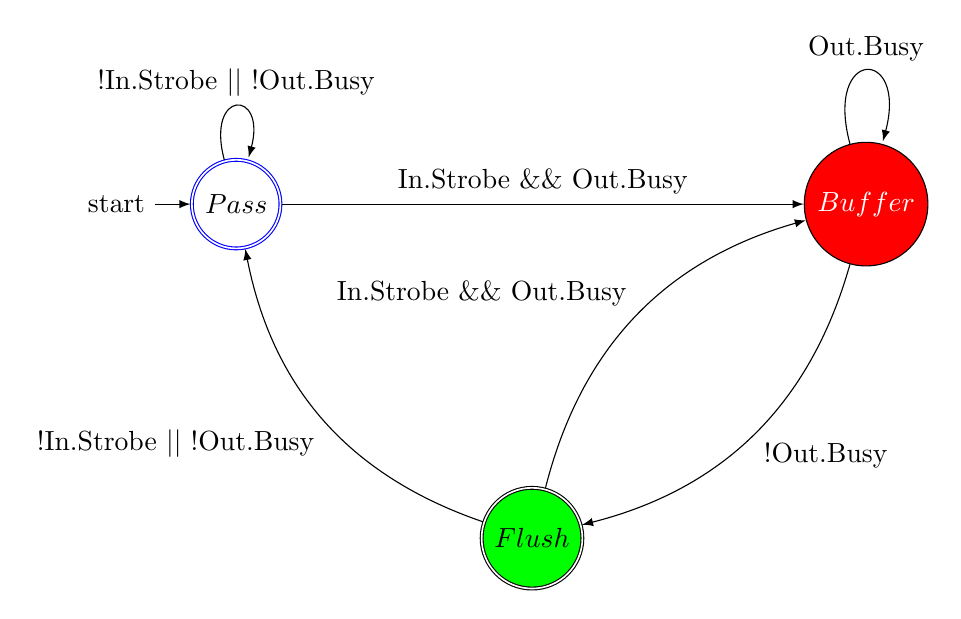
\begin{tikzpicture}[->,>=latex,auto]
    %    \tikzstyle{every node}+=[inner sep=0pt]

        \node[initial,accepting,state,draw=blue] (Pass) {$Pass$};
        \node[state,fill=red,text=white] (Buf) [right of=Pass, node distance=8cm] {$Buffer$};
        \node[accepting,state,fill=green] (Flush) [below left of=Buf, node distance=6cm] {$Flush$};

        \path (Pass)  edge [loop above] node {!In.Strobe $||$ !Out.Busy} (Pass)
                      edge node {In.Strobe \&\& Out.Busy} (Buf)
              (Buf)   edge [loop above] node {Out.Busy} (Buf)
                      edge [bend left] node {!Out.Busy} (Flush) % Bend right
              (Flush) edge [bend left] node {In.Strobe \&\& Out.Busy} (Buf)
                      edge [bend left] node {!In.Strobe $||$ !Out.Busy} (Pass);
        \end{tikzpicture}
        \caption{Handshake State Machine}
    \end{center}
    \label{fig:pipeline-skid-buffer-fsm}
\end{figure}
}

Pipeline stages signal $Busy$ whenever they are in the $Run$ or $Wait$ states.
A circuit is in the $Run$ state while it is processing, and in the $Wait$ state
when it has data sitting on its output but the next stage remains $Busy$.  When
the circuit is neither strobing to the next circuit nor processing, it becomes
$Idle$, and is not $Busy$ even if the next stage becomes $Busy$. This produces
four states:  Idle, Run, Wait, and Finish, shown in
\prettyref{tab:pipeline-exec-circuit-state}.

The circuit passes its data on in the Finish state, and is idle on the next
iteration; however, the busy signal is \inlinecode{Processing || (DataReady
\&\& PipeIn.Busy)}, and so signals \inlinecode{!Busy} on the cycle on which it
delivers data.  The \inlinecode{SkidBuffer} itself must accept the data and,
besides, is \inlinecode{!Busy} when its buffer is empty and will not magically
become busy.

\afterpage{
\begin{table}[ht]
    \caption{Execution Circuit Handshake States} % title of Table
    \centering % used for centering table
    \begin{tabular}{c c c c c} % centered columns (4 columns)
        \hline\hline
        State & Processing & DataReady & PipeOut.Busy & PipeIn.Busy \\ [0.5ex] % inserts table

        \hline
        Idle & 0 & 0 & X & 0 \\
        Run & 1 & 0 & X & 1 \\
        Wait & 0 & 1 & 1 & 1 \\
        Finished & 0 & 1 & 0 & 0 \\ [1ex]
        \hline
    \end{tabular}
    \label{tab:pipeline-exec-circuit-state}
\end{table}
\begin{figure}
    \begin{center}
        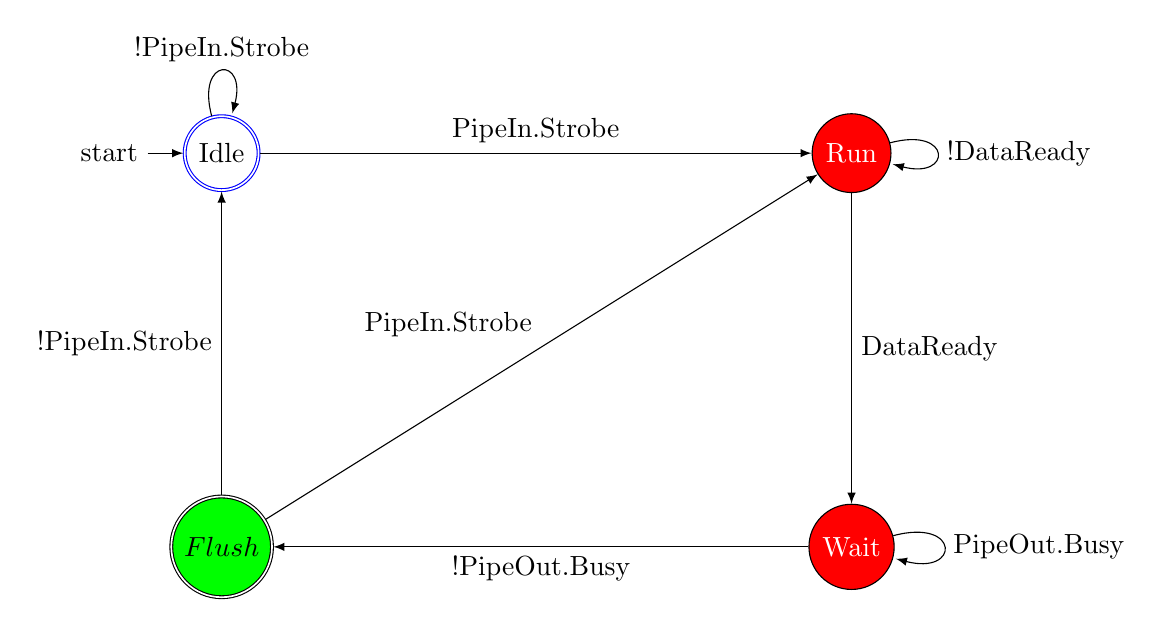
\begin{tikzpicture}[->,>=latex,auto]
            %    \tikzstyle{every node}+=[inner sep=0pt]

            \node[initial,accepting,state,draw=blue,text=black] (Idle) {Idle};
            \node[state,fill=red,text=white] (Run) [right of=Idle, node distance=8cm] {Run};
            \node[state,fill=red,text=white] (Wait) [below of=Run, node distance=5cm] {Wait};
            \node[accepting,state,fill=green] (Finish) [below of=Idle, node distance=5cm] {$Flush$};

            \path (Idle)   edge [loop above] node {!PipeIn.Strobe} (Pass)
            edge node {PipeIn.Strobe} (Run)
            (Run)    edge [loop right] node {!DataReady} (Run)
            edge node {DataReady} (Wait)
            (Wait)   edge [loop right] node {PipeOut.Busy} (Wait)
            edge node {!PipeOut.Busy} (Finish)
            (Finish) edge node {PipeIn.Strobe} (Run)
            edge node {!PipeIn.Strobe} (Idle);
        \end{tikzpicture}
        \caption{Execution Circuit Handshake State Machine}
    \end{center}
\end{figure}
}

\section{Fetch}

The \inlinecode{Fetch} stage obtains new instructions and passes them through
the pipeline.  It can pass forward large amounts of data—64-byte cache
lines—containing several instructions, along with the value of \inlinecode{pc}
after a branch.  \inlinecode{Fetch} always retrieves and passes along a chunk
of instruction stream aligned to its chunk size.


\section{Pre-Decode}

\inlinecode{Pre-Decode} prepares the instruction stream for
\inlinecode{Decode}.  It receives instruction stream from \inlinecode{Fetch}
one chunk at a time, and tracks \inlinecode{pc} to identify the current
address.

\inlinecode{Pre-Decode} converts RISC-V Compressed instructions (RVC) to normal
RISC-V instructions.  RVC includes all opcodes with the two least-significant
bits not equal to \inlinecode{11}, so \inlinecode{Decode} can ignore these two
bits.  This allows cheap handling of \inlinecode{C.JAL} and
\inlinecode{C.JALR}:  RVC passes the lower two bits of the opcode forward
as-is, and the \inlinecode{Branch} circuit adds 2 rather than 4 to
\inlinecode{pc} when these bits are not \inlinecode{11}.

\inlinecode{Pre-Decode} separates each quadrant of RVC into an independent
combinational circuit and selects the output via a mux.

Whether expanded from RVC or passed forward verbatim, \inlinecode{Pre-Decode}
assembles a single 32-bit instruction with its context information for
\inlinecode{Decode}.

\section{Decode}

\inlinecode{Decode} converts instructions to an internal bundle of signals
indicating the operation, width, signed or unsigned nature, and instruction
layout type.  Like \inlinecode{Pre-Decode}, groups of logically-similar
instructions execute as independent combinational circuits and raise a signal
to indicate an identified instruction.

Often a single opcode maps to only one or two formats, and the
\inlinecode{funct3} and \inlinecode{funct7} fields indicate data width, sign,
or modes such as shift-right or subtract, so these circuits are quite compact
in gate logic.  A 5-LUT can decode an opcode, and often a 5-LUT or 6-LUT can
look up the remaining information—often one bit in the opcode, three from
\inlinecode{funct3}, and one from \inlinecode{funct7}.  This minimizes the
logic used on FPGAs.

\section{Dispatch}

\inlinecode{Dispatch} determines if instructions have dependencies on pending
instructions, directs register renaming, and distributes instructions across
multiple execution units if present\footnote{Branches and jumps are always
memory and register barriers; branches cause a stall unless branch prediction
and speculative execution are implemented.  These require additional
checkpointing.  Branches incur a five-cycle stall without prediction, and tight
loops suffer significant loss in IPC.}.

\section{Load}

\inlinecode{Load} loads data from registers and extracts immediate values from
most instructions.  \inlinecode{Execute} derives immediate values from
two-register instructions, notably \inlinecode{Branch} instructions.

\section{Execute}

Small numbers above and below the execute operation indicate the number of
cycles and the latency per execution unit.  For example, if the execution stage
contains two dividers, the latency can be one cycle rather than however long it
takes for the divider to complete.

The \inlinecode{Branch} and \inlinecode{Load/Store} operations use the ALU for
simultaneous addition and comparison.  \inlinecode{Branch} caches the
\inlinecode{pc} and computed address of the prior interpreted branch
instruction, using the cached target address if the branch condition and
\\inlinecode{pc} match\footnote{Speculative adders occasionally run for two
cycles, in which case so will \inlinecode{Load/Store}.  Tight loops use
backwards branches and suffer a significant performance loss if the addition
requires an extra cycle.  The ALU supplies two comparators to allow
simultaneous comparison of \inlinecode{pc} and the branch condition.}.

\inlinecode{Branch} jumps to the the cached target address if the branch
condition and prior branch instruction match, avoiding the adder for all but
the first iteration of a tight loop.  \inlinecode{Branch} flushes the entire
pipeline when taking a non-predicted branch.

\section{Memory Access and Cache}

\inlinecode{Memory Access} also forwards register loads back through the
pipeline.  Both \inlinecode{MemoryAccess} and \inlinecode{Fetch} connect
directly to VC-DSR L1 cache.

At higher clock rates, L1 cache hits may respond in as many as 5 cycles.  A
single cache line holds 64 bits, enough for 16 instructions or 32 compressed
instructions.  Vector instructions can be highly-efficient, using single
full-width execution units to perform operations on multiple smaller-width
data, and fail to saturate the pipeline if it's designed for more than 12
simultaneous operations.  The pipeline can fuse 32-bit instructions in the same
manner, when independent, although this is not implemented.

Instruction fetch thus requires fast trace caching and, more importantly,
highly-efficient branch prediction.

\chapter{Parallelism}

\section{Instruction Level Parallelism}

Kerberos uses a parallel instruction pipeline with multiple execution units.
The Fetch stage obtains several instructions from I\$ and fans them out to
multiple decoder pipelines, which then fan them in to the Dispatch stage as
shown in \prettyref{fig:ilp-pipeline-overview}.

\begin{figure}
    \begin{center}
        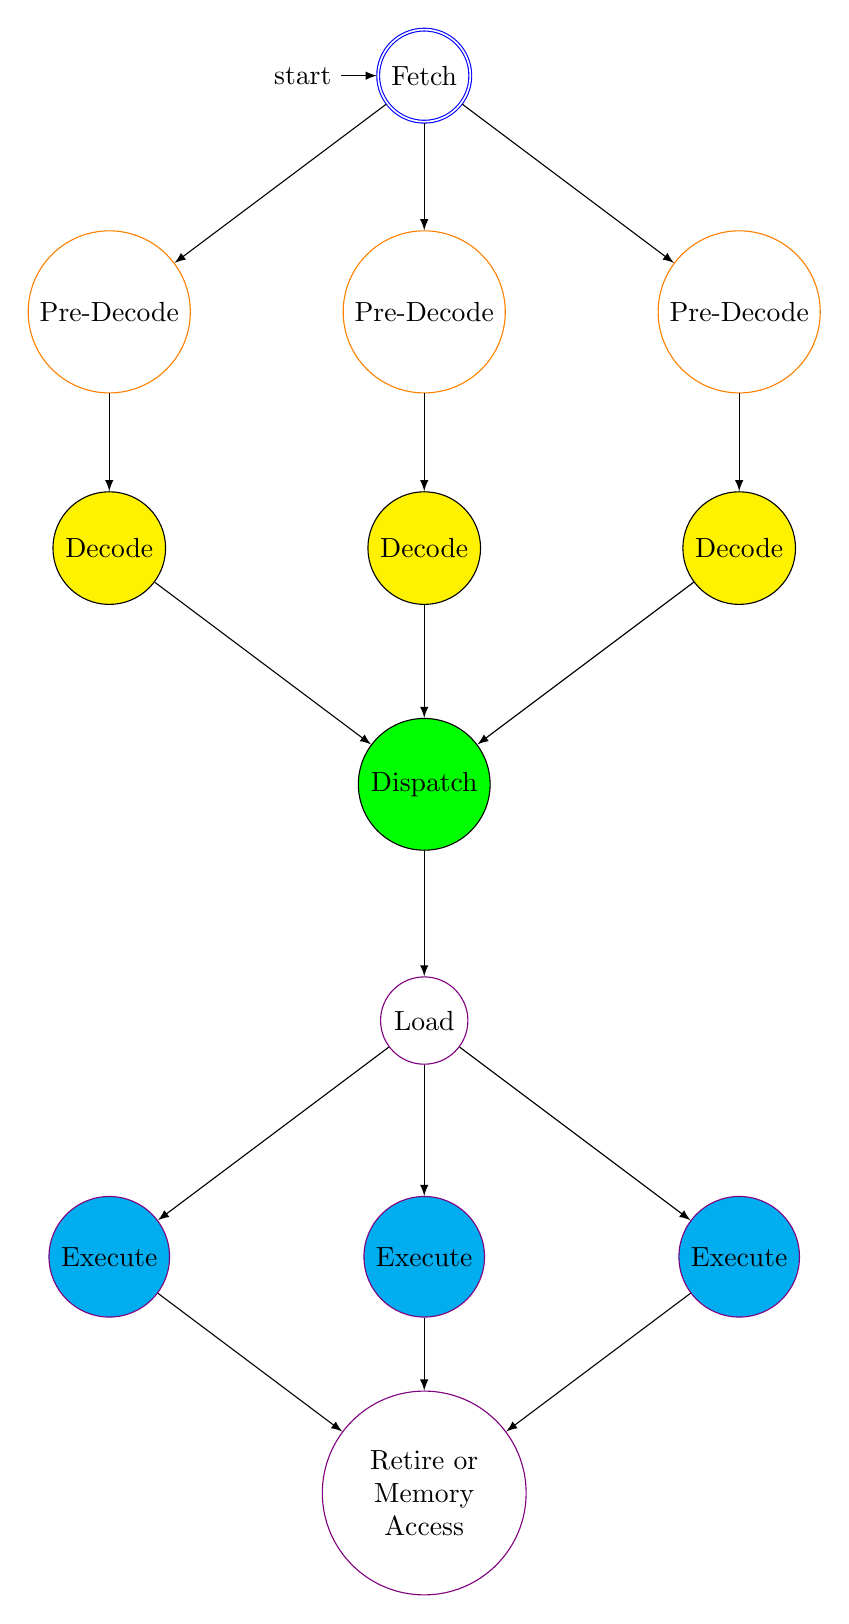
\begin{tikzpicture}[->,>=latex,auto]

        \node[initial,accepting,state,draw=blue] (Fetch) {Fetch};

        \tikzstyle{every node}+=[draw=orange]
        \node[state] (Pre-Decode1) [below of=Fetch, node distance=3cm] {Pre-Decode};
        \node[state] (Pre-Decode2) [left of=Pre-Decode1, node distance=4cm] {Pre-Decode};
        \node[state] (Pre-Decode3) [right of=Pre-Decode1, node distance=4cm] {Pre-Decode};

        \tikzstyle{every node}+=[draw=black,fill=yellow]
        \foreach \x in {1,2,3}
        \node[state] (Decode\x) [below of=Pre-Decode\x, node distance=3cm] {Decode};

        \tikzstyle{every node}+=[fill=white]

        \node[state,fill=green] (Dispatch) [below of=Decode1, node distance=3cm] {Dispatch};

        \node[state,draw=violet] (Load) [below of=Dispatch, node distance=3cm] {Load};

        \tikzstyle{every node}+=[draw=violet,fill=cyan]

        \node[state] (Execute1) [below of=Load, node distance=3cm] {Execute};
        \node[state] (Execute2) [left of=Execute1, node distance=4cm] {Execute};
        \node[state] (Execute3) [right of=Execute1, node distance=4cm] {Execute};

        \tikzstyle{every node}+=[fill=white]
        \node[state] (RMA) [below of=Execute1, node distance=3cm, text width=2cm, align=center] {Retire or Memory Access};

        \foreach \x in {1,2,3}
        \path
            (Fetch) edge (Pre-Decode\x)
            (Pre-Decode\x) edge (Decode\x)
            (Decode\x) edge (Dispatch)
            (Load) edge (Execute\x)
            (Execute\x) edge (RMA);

        \path (Dispatch) edge (Load);

        \end{tikzpicture}
        \caption{Instruction-Level Parallelism Overview}
    \end{center}
    \label{fig:ilp-pipeline-overview}
\end{figure}

Both $Dispatch$ and $Load$ track instruction dependencies; only $Load$ tracks
register contents.  $Dispatch$ determines dependencies and indicates actions
such as register renaming.

When $Dispatch$ executes instructions out of order, it indicates a register ID
from which to read each value and one to which to write any output.  $Dispatch$
delays instructions dependent on a prior write; instructions reading a register
altered by a future write use the prior register ID of that register.  This
allows independent instructions to execute out of order even when using the
same temporary registers.

$Dispatch$ and $Load$ keep a table of registers, their current aliases, and a
\inlinecode{pc} tag.  $Dispatch$ uses the current table to order instructions
and perform renaming, using a free register FIFO.  $Load$ keeps track of
register contents.  Each retiring instruction forwards the relevant information
back so both can keep track of the current register file checkpoint in terms of
\inlinecode{pc}.  The $Retire or Memory Access$ stage also tracks this
information and buffers memory writes to stay in sync with the settled register
checkpoint.

%Instruction-level parallelism

%[I]nstruction, [r-d]estination, [r-s]ource

%Destination = read, source = write


%pc=1000 I rd1, rs2  r1→r1a
%pc=1001 I rd2, rs3  r2→r2a
%pc=1002 I rd3, rs2  r3→r3a, !r2←r2a(1001) [r2a final dependency: 1002]
%pc=1003 I rd4, rs2  r4→r4a, !r2←r2a(1001) [r2a final dependency: 1003]
%pc=1004 I rd5, rs3  r5→r5a, !r3←r3a(1002) [r3a final dependency: 1004]
%pc=1005 I rd2, rs4  r2→r2b, !r4←r4a(1001) [r4a final dependency: 1005] [r2a retired, free after pc = 1003]
%pc=1006 I rd6, rs2  r6→r6a, !r2←r2b(1005) [r2b final dependency: 1006]
%...


% New instruction:  Set read dependency on current source-registers as aliased;
%  Update final dependency on those source registers to current pc
%
% Rename destination register; update alias at current pc to point to destination register
%
% Check read dependency on non-retired data written by prior instructions
%  If dependency, set aside
%  Else, dispatch
%
% Instruction complete:  forward data back to Load; accounting back to Dispatch
%
% Memory access:  Buffer memory writes relative to highest executed pc; signal register checkpoint
% to one instruction prior to lowest non-executed pc and writeback buffer to RAM
%
% NOTE:  Need a fast way to cross-check a set of instructions against one another in parallel.
% Possibly by a first-select MUX to parallel evaluate interdependencies.  Multi-stage is also
% possible for huge instruction-per-clock, but creates a longer pipeline with large IPC costs to
% branch misprediction.


% Horizontal?
%
%      1000 1001 1002 1003
%
% Read   r1   r1   r2   r1
% Write  r2   r3   r4   r5
%
%



\begin{figure}
    \begin{center}
        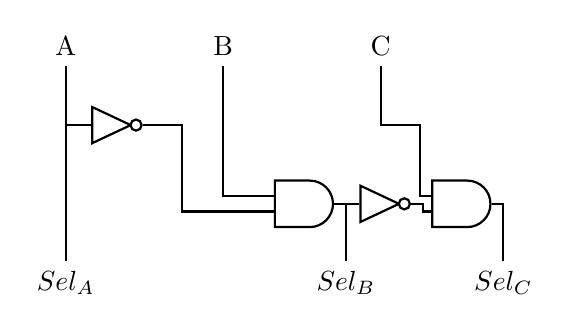
\begin{tikzpicture}[auto]
            \node (A) at (0,0) {A};
            \draw (A) ++(2,0) node (B) {B};
            \draw (B) ++(2,0) node (C) {C};

            \tikzstyle{every node}+=[black, thick, fill=white]
            % AND gate
            \node[and gate US, draw] at ($(B) + (1,-2)$) (BAnd) {};
            \node[and gate US, draw, fill=white] at ($(C) + (1,-2)$) (CAnd) {};
            \node[not gate US, draw, fill=white] at ($(A) + (0.5,-1)$) (ANot) {};
            \node[not gate US, draw, fill=white] at ($(BAnd.output) + (0.5,0)$) (BNot) {};

            \draw (A) ++(0,-3) node (ASel) {$Sel_A$};
            \draw ($(BAnd.output) + (0.15,-1)$) node (BSel) {$Sel_B$};
            \draw ($(CAnd.output) + (0.15,-1)$) node (CSel) {$Sel_C$};
            \path
                [black, draw, thick]
                (A) -- (ASel)
                (A) -- ++(0,-1) |- (ANot.input)
                (ANot.output) -- ++(0.5,0) |- (BAnd.input 2);
            \path
                [black, draw, thick]
                (B) |- (BAnd.input 1)
                (C) -- ++(0,-1) -- ++(0.5,0) |- (CAnd.input 1)
                (CAnd.output) -- ++(0.15,0) -- (CSel);
            \path
                [black, draw, thick]
                (BAnd.output) |- (BNot.input)
                (BAnd.output) ++(0.15,0) -- (BSel)
                (BNot.output) -- ++(0.15,0) |- (CAnd.input 2);

%\path
%[black, draw, thick]
%(SS) ++(2.5,2) |- (SSAnd.input 1)
%(SS) ++(1,2) -- ($(ART) + (1,-8)$)
%(SS) ++(0.5,3.75) -- ++(1,1) % Slash to show multi-data bus
%(LLVP) ++(0,-5.5) |- (SSNot.input) (SSNot.output) -- ++(-0.5,0) |- (SSAnd.input 2)
%(SSAnd.output) -- ($(ART) + (3,-8)$);

        \end{tikzpicture}
\caption{Logical find-first circuit, ripple}
\end{center}
\label{fig:ilp-logical-find-first}
\end{figure}

\begin{figure}
    \begin{center}
        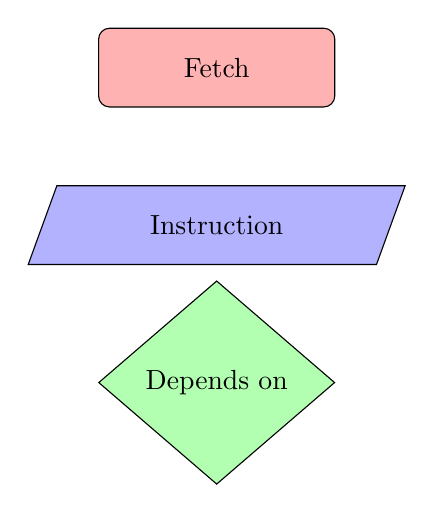
\begin{tikzpicture}[->,>=latex,auto]
            %    \tikzstyle{every node}+=[inner sep=0pt]
            \node (Fetch) [startstop] {Fetch};
            \node (Instruction) [io, below of=Fetch, node distance=2cm] {Instruction};
            \node (WriteBlocked) [decision, below of=Instruction, node distance=2cm] {Depends on};

        \end{tikzpicture}
        \caption{Out-of-Order Execution Flow Chart}
    \end{center}
    \label{fig:ooe-flow-chart}
\end{figure}

\section{Lightweight Vector Operations}

Kerberos provides lightweight vector operations using a custom user CSR.

\begin{figure*}[h!]
    {\footnotesize
        \begin{center}
            \begin{tabular}{U@{}cccc}
                \instbitrange{31}{7} &
                \instbit{6} &
                \instbit{5}{4} &
                \instbitrange{3}{0} \\
                \hline
                \multicolumn{1}{|c|}{\warl} &
                \multicolumn{1}{c|}{E} &
                \multicolumn{1}{c|}{M[1:0]} &
                \multicolumn{1}{c|}{Size[3:0] (\wlrl)} \\
                \hline
                27 & 1 & 2 & 4 \\
            \end{tabular}
        \end{center}
    }
    \vspace{-0.1in}
    \caption{Lightweight Vector Register ({\tt zvinxd}).}
    \label{zvinxreg}
\end{figure*}

Setting ``Size'' to 0 disables vector operations; other values enable vector
operations.

``E'' controls RVE mode and is always supported; ``E'' is always set in RVE
mode and cannot be unset.  When ``E'' is not set, the vector registers are x31
and x19; when ``E'' is set, the vector registers are x15 and x11.  These are
called the high and low vector registers, respectively, and named $vh$ and
$vl$.

``Size'' indicates the number of registers used as vector registers.  Size may
not be greater than 12 when When ``E'' is unset, 8 when ``M'' is non-zero, and
4 when ``E'' is set.  The high and low register sets extend from the high and
low registers down, e.g. if E is unset and Size is 3, the vector registers are
[x31,x30,x29] and [x19,x18,x17],  corresponding respectively.

These relationships also apply to the floating point registers.

When ``M'' is non-zero, x23 acts as a vector mask:  operations only apply to
vector elements where x23[i] is 1.  When ``M'' is 01, vector operations do not
apply to masked vector elements, and the elements are unchanged in the
register, read on load, and written back on store; when ``M'' is 10, vector
operations do not apply to masked elements, and masked elements are zeroed on
load and written back on store; when ``M'' is 11, vector operations do not
apply to masked elements, loads do not overwrite masked elements in the
registers, and stores do not affect the memory contents targeted by masked
elements.

\begin{table}[htp]
    \begin{small}
        \begin{center}
            \begin{tabular}{cl}
                \hline
                \multicolumn{1}{|c|}{M Register} &
                \multicolumn{1}{c|}{Meaning} \\
                \hline
                \multicolumn{1}{|c|}{00} &
                \multicolumn{1}{c|}{No masking}\\
                \hline
                \multicolumn{1}{|c|}{01} &
                \multicolumn{1}{c|}{Load and store masked elements unchanged}\\
                \hline
                \multicolumn{1}{|c|}{10} &
                \multicolumn{1}{c|}{Load masked elements as zero}\\
                \hline
                \multicolumn{1}{|c|}{11} &
                \multicolumn{1}{c|}{Ignore:  loads and stores do not overwrite masked elements}\\
                \hline
            \end{tabular}
        \end{center}
    \end{small}
    \caption{Accrued exception flag encoding.}
    \label{bitdef}
\end{table}

Vector operations are instructions operating on $rd=vh$, $rs1=vh$, $rs2=vl$,
plus load operations with $rd=vh$ or $rd=vl$.  The operations \inlinecode{add},
\inlinecode{sub}, \inlinecode{sll}, \inlinecode{srl}, \inlinecode{sra},
\inlinecode{and}, \inlinecode{or}, \inlinecode{xor}, \inlinecode{slt},
\inlinecode{slti}, all ``M'' extension instructions, \inlinecode{lr} and
\inlinecode{sc} variants, and floating point operations are valid vector
operations; sub-word-size integer operations

Kerberos executes instructions in the given form by expanding them to many
instructions at the current operating width.  For example, after a
\inlinecode{LH x31, offset(rs)} and with $Size=4$ and $S=1$ on RV64, an $add
x31, x31, x19$ will add each of 16 values each 16-bits wide and packed 4 per
register across $x19$ through $x16$ to the current values in $x31$ through
$x28$, storing in the latter.  Other values of $rd$, $rs1$, and $rs2$ have no
special effect.  If the load were $LW$, it would operate on the two sets of 8
values each 32-bits wide.

This allows Kerberos to load a large amount of data into two sets of registers,
perform large numbers of calculations split across large numbers of execution
units, and write those values back to main memory in single instructions.  When
not holding vector data, writes to any register other than $x31$ (and for loads,
other than $x19$ as well) and operations not between $x31$ and $x19$ with
result stored in $x31$ operate as normal.

All registers below the upper vector range are available for program logic use
immediately after a vector instruction, as well as all between $x19$ and the
lowest upper vector register:  the result is in the upper vector range, and likely
is intended to be written out.  Likewise, because Load and Store only operate
on the upper or lower vector registers, large \inlinecode{memcpy} operations can
use 12 registers at once—96 bytes per instruction for Load and Store, which can
bypass execution units.

Program logic using lightweight vector extensions must test for vector behavior,
possibly by executing a two-register-wide vector \inlinecode{AND} with zero in
$x19$ and $x18$ and with non-zero loaded to $x30$, and then checking if x30 has
changed.  If no change, program behavior must account for no vector extension.

Kerberos achieves this internally by dispatching vector instructions as multiple
regular instructions, tagged for width as normal, with the same \inlinecode{pc}
an an indication of their vector index in the register.  Computed values are
reassembled into full instructions.  \inlinecode{and, or, xor} can operate on
entire registers at once with a single execution unit; \inlinecode{sll, srl,
sra} require an extra cycle to mask the shifted-out bits.

\inlinecode{add, sub} require modified adders able to produce results without
further carry at intermediate stages, or else will occupy many execution units.
These remove several intermediate stages, and all intermediate stages at the
beginning of each word.  A 64-bit adder built in this manner can perform eight
8-bit, four 16-bit, two 32-bit, and one 64-bit addition or subtraction
simultaneously with minimal additional hardware, with the original 64-bit path
being the critical path.

These optimizations allow one vector register to operate on one execution unit,
such that a 12 64-bit register vector addition can produce 96 additions on 12
execution units simultaneously.  Multiple vector instructions can only occur in
parallel in the same pipeline with SMT; on the other hand, a pipeline
provisioned for SMT can make good optimistic use of a non-full pipeline via
vector instructions.

\section{Simultaneous Multi-Threading}

Extending the above, Kerberos can include multiple register files and tracking
data structures on a single pipeline.  $Fetch$ tags each instruction with a
thread ID, and all computations use tables, buffers, and register data
associated with that thread ID.

The operating system can schedule multiple running processes on a single
execution core, with some performance impacts from shared cache resources.
Proper use of Address Space IDs (ASIDs) is critical to keep L1 cache properly
separated.  When only one process is scheduled on a single core, all execution
units are available for use.

\chapter{Cache Mechanisms}

Caching faces complex concerns:  delay, synonym detection, the precise manner
of tagging, security issues such as seen in recent speculative execution
vulnerabilities, and more.

\section{NCOR}

In 2012, Aasaraai and Moshovos published "NCOR:  An FPGA-Friendly Nonblocking
Data Cache for Soft Processors with Runahead Execution."  Nonblocking cache
allows instruction-level parallelism and specifically allows runahead
execution, wherein a CPU waiting for a cache miss—possibly long enough to
execute several tens or hundreds of instructions—can run instructions with
incorrect data and discard the results just to figure out what data will be
fetched.  A load-store architecture like RISC-V accesses memory infrequently
while executing, so long as the instruction cache can provide the next several
instructions.  Runahead discards the results of instructions, but queues data
cache loads as best it can predict so they occur while the CPU executes
preceding instructions.  Runahead can often generate confirmed correct
computations, notably for branches, providing a high-accuracy branch predictor.

Runahead does particularly interesting things when encountering loops:  if it
can properly predict valid load addresses within the loop—such as by tracking
an increment—it can rapidly identify further data with high accuracy.  If
runahead produces erroneous results, a cache miss will occur when entering the
loop; once inside the loop, this information is definitely correct, and
runahead generally predicts the correct results.

NCOR provides a non-blocking cache which avoids content-addressable memory and
leverages FPGA resources such as BRAM.  It reaches fMax of over 325MHz on a
Spartan III with a 4KiB cache, versus 200MHz for a stripped-down MSHR-based
cache.  Both architectures spend more time slogging through larger caches, with
NCOR running at 300MHz on both 8KiB and 16KiB cache sizes, and near 275MHz on
32KiB.  Separate instruction and data caches with slower (multi-cycle, low
delay but longer latency) L2 cache allow higher fMax when the cache
infrastructure is in the critical path, which means more runahead distance and
fewer cache misses.

\section{VC-DSR}

Most L1 caches are virtually-indexed, physically-tagged (VIPT).  This requires
a TLB lookup on each cache access, possible page table walking, and other slow
behavior.  The TLB lookup itself induces longer delays.  Virtually-indexed,
virtually-tagged (VIVT) caches can encounter multiple virtual addresses (VAs)
with the same physical address, called synonyms.

Yoon and Sohi proposed\footcite{Yoon2016} a Virtual Cache with Dynamic Synonym
Remapping (VC-DSR), as shown in \prettyref{fig:VC-DSR}.  This solves the
synonym probleh in VIVT by looking up synonyms in an Active Synonym Table (AST)
if a virtual address matches a Synonym Signature (SS), implemented as a bloom
filter.  If no SS or AST hit, it checks the VC as normal.  When multiple cached
virtual pages map to the same physical page, the AST provides the Leading
Virtual Page (LVP) used to look up the address in the VC, as well as the
permissions and other metadata for that particular virtual page.  The cache
then looks up the tag for the leading virtual page—logically, it replaces the
bits in the virtual address with the bits of the leading virtual page,
producing the Leading Virtual Address (LVA), and uses that to find the cache
line; the L1 arbiter ignores the metadata in this cache entry, using the data
from the AST instead.

\begin{figure}[hbpt]
    \centering
    \includegraphics[width=\textwidth]{images/VC-DSR_Cache}
    \caption{\label{fig:VC-DSR}VC-DSR as diagramed by Yoon and Sohi, with LLVP added.}
\end{figure}

On VC miss, the TLB checks the Active Synonym Detection Table (ASDT) to
determine if the virtual page is known to correspond to a physical page in
cache.  If not, the caching system makes further requests to L2 cache or
performs a page table walk.  If the virtual page ultimately does reference a
physical page already in cache, the cache arbiter hashes the page, sets the
corresponding bit in SS, increments a counter for this bit, and inserts the
virtual page into the AST as a synonym to the LVP.

The Last LVP (LLVP) optimization, shown in \prettyref{fig:VC-DSR}, stores the
last leading virtual page and requested page in a register, along with
metadata.  If the requested address matches the last requested address, the
cache arbiter can immediately check metadata (read or write permission) and mux
the LVP from this register.  Consecutive memory accesses to the same synonym
page skip the AST check; the SS check occurs in parallel, but adds no delay and
has no effect.

RISC-V provides a Global bit in the PTE.  The cache arbiter ignores the ASID
for Global pages, placing no entry in the SS or AST for the same virtual page
in different ASIDs.  Synonyms mapped at alternate virtual addresses are treated
as normal.  On IA-32 and AMD64, Yoon and Sohi assume the top half of virtual
address space is global.

% vim: ts=4 sw=4 et
\chapter{Speculative Execution}

This chapter covers speculative execution.

\section{Security}

Speculative execution causes side effects:

\begin{itemize}

    \item Cache is loaded or invalidated

    \item Branch prediction tables are updated

\end{itemize}

These side effects are usually harmless.  Runahead, for example, continues
executing during a D\$ miss to speculatively load the cache.  Because the
registers and memory buffer contain no privileged information, runahead can't
access any information not available to the thread normally, and so cannot leak
information.

These guarantees fail when processors contain severe design flaws.

\subsection{Impermissible Cache Loads}

Meltdown leverages impermissible loads by using the data as an offset into an
uncached memory area and searching for a statistically-fast read indicating
cached data.  Meltdown relies on speculative execution issuing these reads
after accessing a supervisor page.

Kerberos's VC-DSR stores the ASID and permissions for each cache line's leading
virtual page and for each virtual page synonym to the leading virtual page.
D\$ does not provide instructions to the pipeline, so these permissions include
only R, W, and U.  Any load or store operation must supply the ASID and whether
it's reading or writing; adding the U bit allows Kerberos to short-circuit a
data load in a number of ways:

\begin{itemize}

    \item A D\$ hit finds a permission mismatch, and D\$ returns a protection
        fault

    \item A D\$ miss finds an entry in the ART, TLB, or ASDT with a permission
        mismatch, and D\$ returns a protection fault

    \item A D\$ TLB miss causes a page table walk and finds a permission
        mismatch, and D\$ returns a protection fault

\end{itemize}

\subsection{L1 Cache Address Translation}

Modern caches are virtually-indexed, physically-tagged (VIPT), and need to look
up physical addresses in certain situations.  This mechanism in particular
caused Foreshadow and Foreshadow-NG, where a program reads arbitrary data from
L1 cache before the tag is resolved.

Kerberos uses a VIVT cache and isn't subject to this.

\begin{itemize}

    \item Cache line tags include ASID and, for hypervisor extensions, VMID,
        associating them with an address space context to avoid homonyms.

    \item Synonyms aren't even vaguely related to the index and tag they
        reference, so speculation ahead of an ART lookup would be bizarre.

    \item Repeated access to the same page uses a LLVP register to avoid the
        ART and avoid the SS false positive condition; a larger SS dramatically
        reduces the false positive rate, while speculating in the manner by
        which Foreshadow occurs would be enormously more expensive.

    \item Global pages bypass ART in that ASIDs aren't factored into their
        synonym check.

    \item Physical address information must be looked to determine if an L1
        miss is real, and is available for L2 lookups, at which point no
        further misreads are possible.

\end{itemize}

Because of all this, VC-DSR cannot function in a manner by which speculative
cache fetches provide any use.

\subsection{Store Bypass}

A store buffer contains only data from the current context and cannot contain
impermissible data.  Specter Speculative Store Bypass (SSB) leverages
misaligned loads and stores to pull
rogue system register read

\subsection{Branch Speculation}

{\bf FIXME:  very rough, mostly tacked down as scribbled notes}

Spectre leverages branch misprediction and speculative execution.

Fully-associative caches do not correlate the specific cache line with a
specific address due to not being indexed.

Number of evicted cache lines is abusable:

\begin{itemize}

    \item Mispredict branch

    \item Load register

    \item begin speculating using register

    \item Start looping through data using register counter

    \item Drop results, take correct branch

    \item Loop through a previously-cached array in reverse and detect last
        cached address

\end{itemize}

Speculation must wait for D\$ to accurately load the register; and further
reads and computations require cached data.  If the data is in cache, this
attack doesn't work; if the data is not in cache, further execution requires
loading the data for accurate results.

During a D\$ miss, Kerberos enters runahead mode, tracking valid and invalid
register and store buffer data and using this to predict valid and invalid
state.  Invalid state may later be proven valid.  Crucially, a predicted branch
is speculative until computed and confirmed.

One of two things will happen during runahead:  the branch will be computed and
the runahead path will be invalidated, or the branch will be computed and the
runahead path will be as valid as it can be in non-branching code.  If the
branch is invalidated, all loads are not valid; if it is validated, {\em some}
loads are valid.

Runahead and speculative execution operate on this principle:  runahead skips
loads and marks registers as not valid when the loads are not known valid,
while speculation notates the results of operations and if they're on
known-valid data.  In Kerberos, runahead doesn't queue up loads in D\$; rather
it queues {\em speculative} loads and flags a validity condition in a bitfield.
When the validity condition is proven true, D\$ performs the load.

For example:  runahead passing a predicted branch will mark all queued loads as
predicated on a validity condition.  When execution proves the branch is
taken—such as after a register load completes and the branch requiring it is
immediately computed to verify the prediction—runahead signals D\$ that the
validity condition is proven.  D\$ will then evict cache lines and load data.

This approach must meet the following constraints:

\begin{itemize}

    \item D\$ has a queue of known-valid items that {\em will} be loaded in the
        execution path, so loading them is harmless.

    \item D\$ does not load or invalidate cache lines until it has a {\em
        valid} address to load.  This means branches leading to the read are
        100\% determined to be taken or not taken, registers used to calculate
        addresses are 100\% determined to contain the expected contents, and so
        forth.

    \item D\$ may issue speculative TLB and ASDT lookups for addresses not in a
        currently-cached LVP, but won't issue these for addresses in a
        currently-cached LVP.  These speculative lookups cannot be used until
        {\em one} address in the referenced virtual page is made valid in L1
        cache, as after the item is valid there is no remaining timing attack
        against the TLB and ASDT.

    \item When a constraint is proven incorrect, D\$ invalidates all related
        queued speculative loads.
\end{itemize}

When a constraint is proven incorrect, no further action is needed except the invalidation of queued speculative loads.  This can be done by simply never validating them {\em if} runahead validity state is managed, which is necessary for this approach.

The processor must indicate the correct computations for upcoming branches to runahead even when runahead isn't running; it must forward valid loads and their source addresses for runahead to compare with its predictions; and so forth.  For a lazy approach, access to a speculative D\$ load must trigger runahead, which then {\em confirms} its validity conditions in a 100\% accurate manner, updates the D\$ speculative queue, and continue runahead using the more-valid state.

This approach ensures CPU behavior can leak state of which the processor was certain, but no information about state of which the processor was uncertain.  Two factors guarantee this:

\begin{itemize}

    \item Prefetch operations such as runahead must not evict cache data not
        yet used by a pending operation to prefetch a cache line used in a
        later operation—this would cause cache misses and decrease
        performance—so software cannot identify future state by looking for
        unexpected cache misses

    \item No cached information shall be used until it is confirmed
        non-speculative, so software can only determine future state from state
        it already has carried out to its correct conclusion, which is what
        software does.

\end{itemize}

This has odd implications, e.g. an incorrectly-predicted loop attempting to
read through an array to extract timing from future execution will remain
marked as speculative and then determined mispredicted, and the timing effects
of cache speculation won't arise.  As soon as the loop is entered, the
misprediction leads to a cache miss which triggers runahead and rapidly loads
cache with correct data.  If the loop is small, it may validate future data and
cause further prefetching, but by nature this can only occur with
confirmed-valid state.

This approach retains the benefits of speculation and prevents the information
leaks brought on by branch misprediction.

\section{Branch Prediction}

Three-block fetch with expensive, complicated, and power-hungry L\$ can fill in
for this when using a good branch predictor.  Modern processors use a trace
cache to bridge between branches, following the same instructions across cache
lines through a much simpler and faster buffer containing a program-order copy
of the reassembled instruction stream; this performs little if any better than
perfect branch prediction when the branch target hits the fetch stage just in
time, but branch predictors aren't perfect.

Kerberos uses a lightweight hybrid predictor consisting of an agree predictor,
a prioritized runahead buffer, and a static predictor.  It also provides a loop
predictor, which identifies when a backwards branch target address is greater
than or equal to the next branch instruction; and an indirect branch predictor
which calculates the target of \lstinline!jalr!.  Unconditional branches are
not tracked in any predictor.

Kerberos considers indirect branches computable when there are several
instructions between \lstinline!jalr rd, n(rx)! and the most recent instruction
setting \lstinline!rx!.  The branch predictor computes this in parallel and
stores it into a one-entry indirect branch register.  When the indirect branch
register

--using a 16-bit parallel prefix adder tied to a carry-select high-speed increment chain—the selectable alternative is the input value and there is a mux for every 16 bits to finish roughly in time

The agree predictor XORs the output of a global shared predictor and a local
predictor to determine strong (0) or weak (1) prediction, as below.

\begin{table}[htp]
    \centering
\begin{tabular}{|c|c|c|}
    \hline
    \multicolumn{2}{|c|}{Predictors} & Prediction \\
    \hline
    Gshare & Local & Agree \\
    \hline
    0 & 0 & Not Taken \\
    \hline
    0 & 1 & Weak Taken \\
    \hline
    1 & 0 & Weak Taken \\
    \hline
    1 & 1 & Taken \\
    \hline
\end{tabular}
\caption{Agree predictor}
\label{tab:branch-agree-predictor}
\end{table}

The static predictor uses the direction to predict the branch.  When the agree
predictor produces a weak-taken result, the static predictor breaks the tie by
using a direction heuristic.

\begin{table}[htp]
    \centering
\begin{tabular}{|c|c|c|}
    \hline
    Agree & Direction & Prediction \\
    \hline
    Taken & Forward & Taken \\
    \hline
    Taken & Backward & Taken \\
    \hline
    Weak Taken & Forward & Not Taken \\
    \hline
    Weak Taken & Backward & Taken \\
    \hline
    Not Taken & Forward & Not Taken \\
    \hline
    Not Taken & Backward & Not Taken \\
    \hline
\end{tabular}
\caption{Predictions accounting for branch direction}
\label{tab:branch-static-hybrid}
\end{table}

Finally, the runahead predictor provides information.  Branches followed using
values from only valid registers are considered definitely taken or not taken;
branches followed using not-valid registers are considered weakly taken or not
taken.

\begin{table}[htp]
    \centering
    \begin{tabular}{|c|c|c|}
        \hline
        Agree & Runahead & Prediction \\
        \hline
        Strong Prediction & Strong Prediction & Runahead \\
        \hline
        Weak Taken & Strong Prediction & Runahead \\
        \hline
        Weak Taken & Weak Taken & Taken \\
        \hline
        Weak Taken & Weak Not Taken & Static \\
        \hline
        Strong Prediction & Weak Prediction & Agree \\
        \hline
        Strong Prediction & No Prediction & Agree \\
        \hline
        Weak Taken & No Prediction & Static \\
        \hline
    \end{tabular}
\caption{Predictions including runahead}
\end{table}

\subsection{Global Shared Predictor}

The global shared predictor (Gshare) uses an 8- to 12-bit Branch History Table
(BHT) providing 256 to 4096 entries in 64 to 1024 bytes of storage.

When a branch is encountered, the lower bits of \lstinline!pc<<2! are XOR'd
with a branch history register (BHR) containing the branch history to create a
BHT index.  The predictor updates the two-bit BHT entry at this index, shifts
the register is shifted one left and the LSB set to the branch outcome, and the
two-bit Smith entry in the BHT update

\subsection{Two-Level Adaptive}

The Yeh algorithm is an option in place of Gshare, and can be much more
accurate with large pattern tables.  The predictor for Yeh uses a pattern
history table (PHT) and a Per-Address History Register Table (PHRT).


\begin{figure}
% Kerberos overview, similar to Taiga diagram
    \begin{center}
        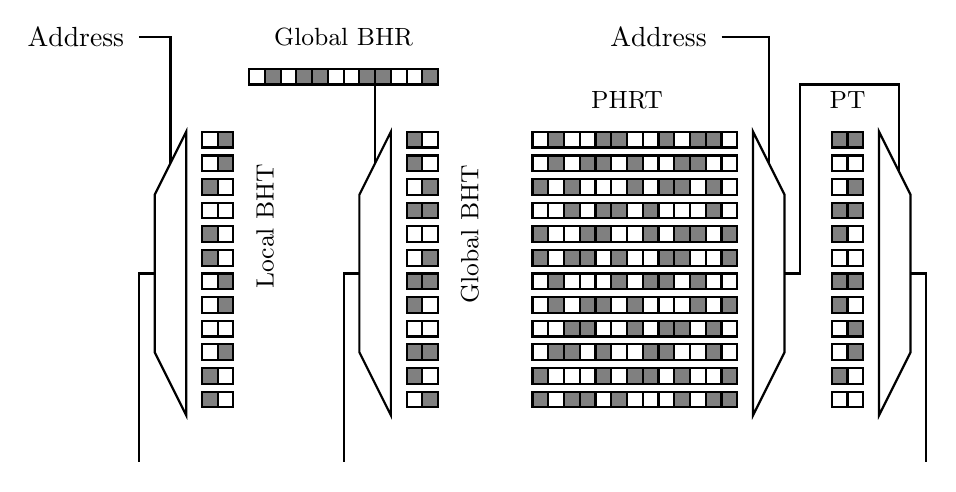
\begin{tikzpicture}[scale=0.2]
            \tikzstyle{every node}+=[inner sep=0pt]

            % Global BHR
            \path
                 % Node and label
                 [black,draw,thick]
                 % Origin
                 (0,0) node [black] (Global BHR) {}
                 ++(6,2) node {\small{Global BHR}};
            % Shift register
            \foreach \x in {0,...,11}
                \path [black, draw, thick]
                 (Global BHR) ++(\x,0) -- ++(1,0) -- ++(0,-1) -- ++(-1,0) -- ++(0,1) -- cycle;
             % Grey boxes
             \foreach \x in {1,3,4,7,8,11}
                \path [black, draw, thick, fill=gray]
             (Global BHR) ++(\x,0) -- ++(1,0) -- ++(0,-1) -- ++(-1,0) -- ++(0,1) -- cycle;

            \path
                [black,draw,thick]
                (Global BHR) ++(18,-4) node (PHRT) {}
              ++(6,2) node {\small{PHRT}};
            \path
                [black,draw,thick]
                (PHRT) ++(18,0) node (PT) {}
              ++(2,2) node {\small{PT}};

            \path
                [black,draw,thick]
                (Global BHR) ++(-3,-4) node (Local BHT) {}
                ++(4,-6) node [rotate=90]{\small{Local BHT}};

            % Local BHT
            \path
                [black,draw,thick]
                (Global BHR) ++(10,-4.5) node (Global BHT) {}
              ++(4,-6) node [rotate=90]{\small{Global BHT}};
            \foreach \y in {0,...,11}
                \foreach \x in {0,1,13,14,21,22,...,33,40,41}
                  \path [black, draw, thick]
                  (Local BHT)
                ++($(\x,0) + -1.5*(0,\y)$)
                  -- ++(1,0) -- ++(0,-1) -- ++(-1,0) -- ++(0,1) -- cycle;

%            \foreach \y in {0,...,11}
%                \foreach \x in {14,...,15}
%                \path [black, draw, thick]
%                (Local BHT)
%              ++($(\x,0) + -1.5*(0,\y)$)
%                -- ++(1,0) -- ++(0,-1) -- ++(-1,0) -- ++(0,1) -- cycle;

            %%%%%% All this to make it look random
            \foreach \y in {0,...,11}
                \foreach \x in {0,1,13,14,21,22,...,33,40,41}
                \ifthenelse{
                   \intcalcMod{
                     \intcalcAdd{
                      \x}{
                      \intcalcMul{\y}{7}
                     }
                   }{3}
                > 0 \AND
                \intcalcMod{
                    \intcalcAdd{
                        \y}{
                        \intcalcMul{\x}{11}
                    }
                }{7} > 1
            }{
                  \path [black, draw, thick, fill=gray]
                    (Local BHT)
                ++($(\x,0) + -1.5*(0,\y)$)
                -- ++(1,0) -- ++(0,-1) -- ++(-1,0) -- ++(0,1) -- cycle}{};
            %%%%% Never try to read that ugly code

        \path
            [black,draw,thick]
            (Local BHT) ++(-1,0)
            -- ++(0,-18) -- ++(-2,4) -- ++(0,10) -- ++(2,4) -- cycle
            (Local BHT)
          ++(-8, 6) node {Address};
        \path
            [black,draw,thick]
            (Global BHR) ++(9,-4)
            -- ++(0,-18) -- ++(-2,4) -- ++(0,10) -- ++(2,4) -- cycle;
        \path
            [black,draw,thick]
            (PHRT) ++(14,0)
            -- ++(0,-18) -- ++(2,4) -- ++(0,10) -- ++(-2,4) -- cycle
            (PHRT)
          ++(8,6) node {Address}
            (PT) ++(4,0)
            -- ++(0,-18) -- ++(2,4) -- ++(0,10) -- ++(-2,4) -- cycle;
        %%%% MUX traces
        \path
            [black,draw,thick]
            (Local BHT) ++(-3,-9)
            -- ++(-1,0) -- ++(0,-12)
            (Global BHR) ++(7,-13)
            -- ++(-1,0) -- ++(0,-12)
            (PHRT) ++(16,-9);
        \path
            [black,draw,thick]
            (Local BHT) ++(-4,6)
            -- ++(2,0) -- ++(0,-8);
        \path[black,draw,thick]
            (Global BHR) ++(8,-1)
            -- ++(0,-5);

        \path
            [black,draw,thick]
            (PHRT) ++(16,-9)
            -- ++(1,0) -- ++(0,12) -- ++(6.25,0) -- ++(0,-5.5)
            (PHRT) ++(24,-9)
            -- ++(1,0) -- ++(0,-12);
        \path
            [black,draw,thick]
            (PHRT) ++(16,-9)
            -- ++(1,0) -- ++(0,12) -- ++(6.25,0) -- ++(0,-5.5)
            (PHRT) ++(24,-9)
            -- ++(1,0) -- ++(0,-12);
        \path
            [black,draw,thick]
            (PHRT) ++(12,6)
            -- ++(3,0) -- ++(0,-8);
        \end{tikzpicture}
    \caption{Three branch predictors.  From left to right:  One-level predictor; Gshare; and two-level Yeh predictor.  12-bit wide registers are shift registers keeping the branch history.  An Agree predictor may branch when two or more different predictors agree.}
    \end{center}
    \label{fig:Kerberose-yeh_branch_predictor}
\end{figure}



Whereas Gshare hashes the branch address with the branch history to look up
history in a global BHT, Yeh looks up the branch address in a table and tracks
its own branch history there—a local branch predictor.

\backmatter
% bibliography, glossary and index go here.
%\printbibliography
\end{document}